\documentclass[a4paper,12pt]{article}
\usepackage[utf8]{inputenc}
\usepackage{array}
\usepackage[left=20mm,top=20mm,right=20mm,bottom=20mm]{geometry}
\usepackage{tabularx}
\usepackage{longtable}
\usepackage[pdftex]{graphicx}
\usepackage{xcolor}
\usepackage{textcomp}
\usepackage{gnuplot-lua-tikz}
\usepackage{tikz}
\usepackage{amssymb}
\usepackage{cite}
\usepackage{hyperref}
\usepackage{soul}
% \usepackage{lineno}
\usepackage[ruled,norelsize]{algorithm2e}
\usepackage{listings}


%opening
\title{Qucs-S: Getting started analog simulation with Ngspice backend}
\author{Vadim Kuznetsov}

\begin{document}

\maketitle

%\begin{abstract}

%\end{abstract}

\section{Introduction} \label{sec:intro}

Qucs-S was forked from the Qucs cross-platform circuit simulator in 2017. "S" letter indicates SPICE. The purpose of the Qucs-S subproject is to use free SPICE circuit simulation kernels with the Qucs GUI. It merges the power of SPICE and the simplicity of the Qucs GUI. Qucs intentionally uses its own SPICE incompatible simulation kernel Qucsator. It has advanced RF and AC domain simulation features, but most of the existing industrial SPICE models are incompatible with it. Qucs-S is not a simulator by itself, but requires to use a simulation backend with it. The schematic document format of Qucs and Qucs-S are fully compatible. Qucs-S allows to use the following simulation kernels with it:

\begin{itemize}
 \item  Ngspice is recommended to use. Ngspice is powerful mixed-level/mixed-signal circuit simulator. The most of industrial SPICE models are compatible with Ngspice. It has an excellent performance for time-domain simulation of switching circuits and powerful postprocessor.
 \item XYCE is a new SPICE-compatible circuit simulator written by Sandia from the scratch. It supports basic SPICE simulation types and has an advanced RF simulation features such as Harmonic balance simulation.
 \item SpiceOpus is developed by the Faculty of Electrical Engineering of the Ljubljana University. It based on the SPICE-3f5 code.
 \item Qucsator as backward compatible and for RF simulation with microwave devices.
\end{itemize}

Qucs-S is a cross-platform software and supports a number of Linux distributions alongside with Windows\texttrademark. The Linux packages are generated automatically with the Open Build Service (OBS ) system. Check the official website to get the list of supported distributions. Please keep in mind that the installation packages doesn't provide the simulation kernel. It need to be installed separately. The Ngspice is recommended. For Debian and Ubuntu it is installed automatically as the dependency. Refer to Ngspice website for installation instructions for other platforms.

\section{Setup on the first start}

Once the Qucs-S is installed, it asks to select the simulation kernel. Since the version 2.0.0 the application tries to find Ngspice in some usual system locations on the first start. If the Ngspice executable was found automatically the information message will be shown. Otherwise the user will be prompted to configure the simulators manually. The following window (Fig. \ref{fig:sim_setup}) is opened after the first start  of the application. Select the default simulator using the drop-down list and correct the simulator executable paths if necessary. These settings could be corrected later using the \textit{Simulation}\verb|->|\textit{Select default simulator} menu. 

\begin{figure}[!ht]
  \begin{center}
    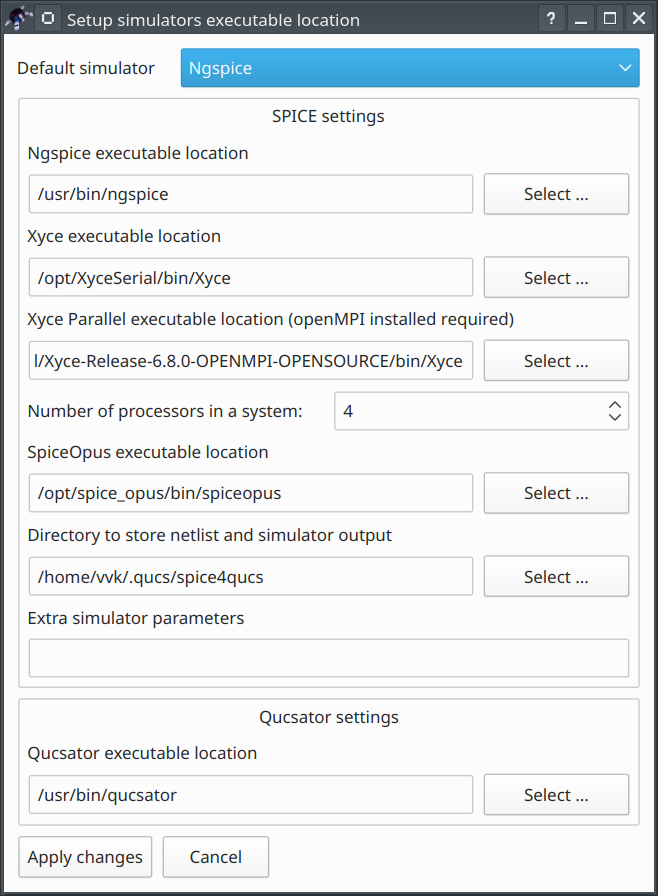
\includegraphics[width=0.4\textwidth]{img/sim_setup.png}
  \end{center}
  \caption{Simulator setup dialog} \label{fig:sim_setup}
\end{figure}

Quick switching of the simulation kernel without application restart is supported since version 2.0.0. See the section \ref{sec:quick_sw} for more details.

\section{Main window structure}


The Qucs-S main window is shown in the Fig. \ref{fig:mainwin}. The main window consists of two areas: schematic editor (4) on the right side and main dock (1) on the left side. Several schematics could be opened simultaneously. It's possible to switch between the opened schematics using the tabular bar above the schematic editor area.    

\begin{figure}[!ht]
  \begin{center}
    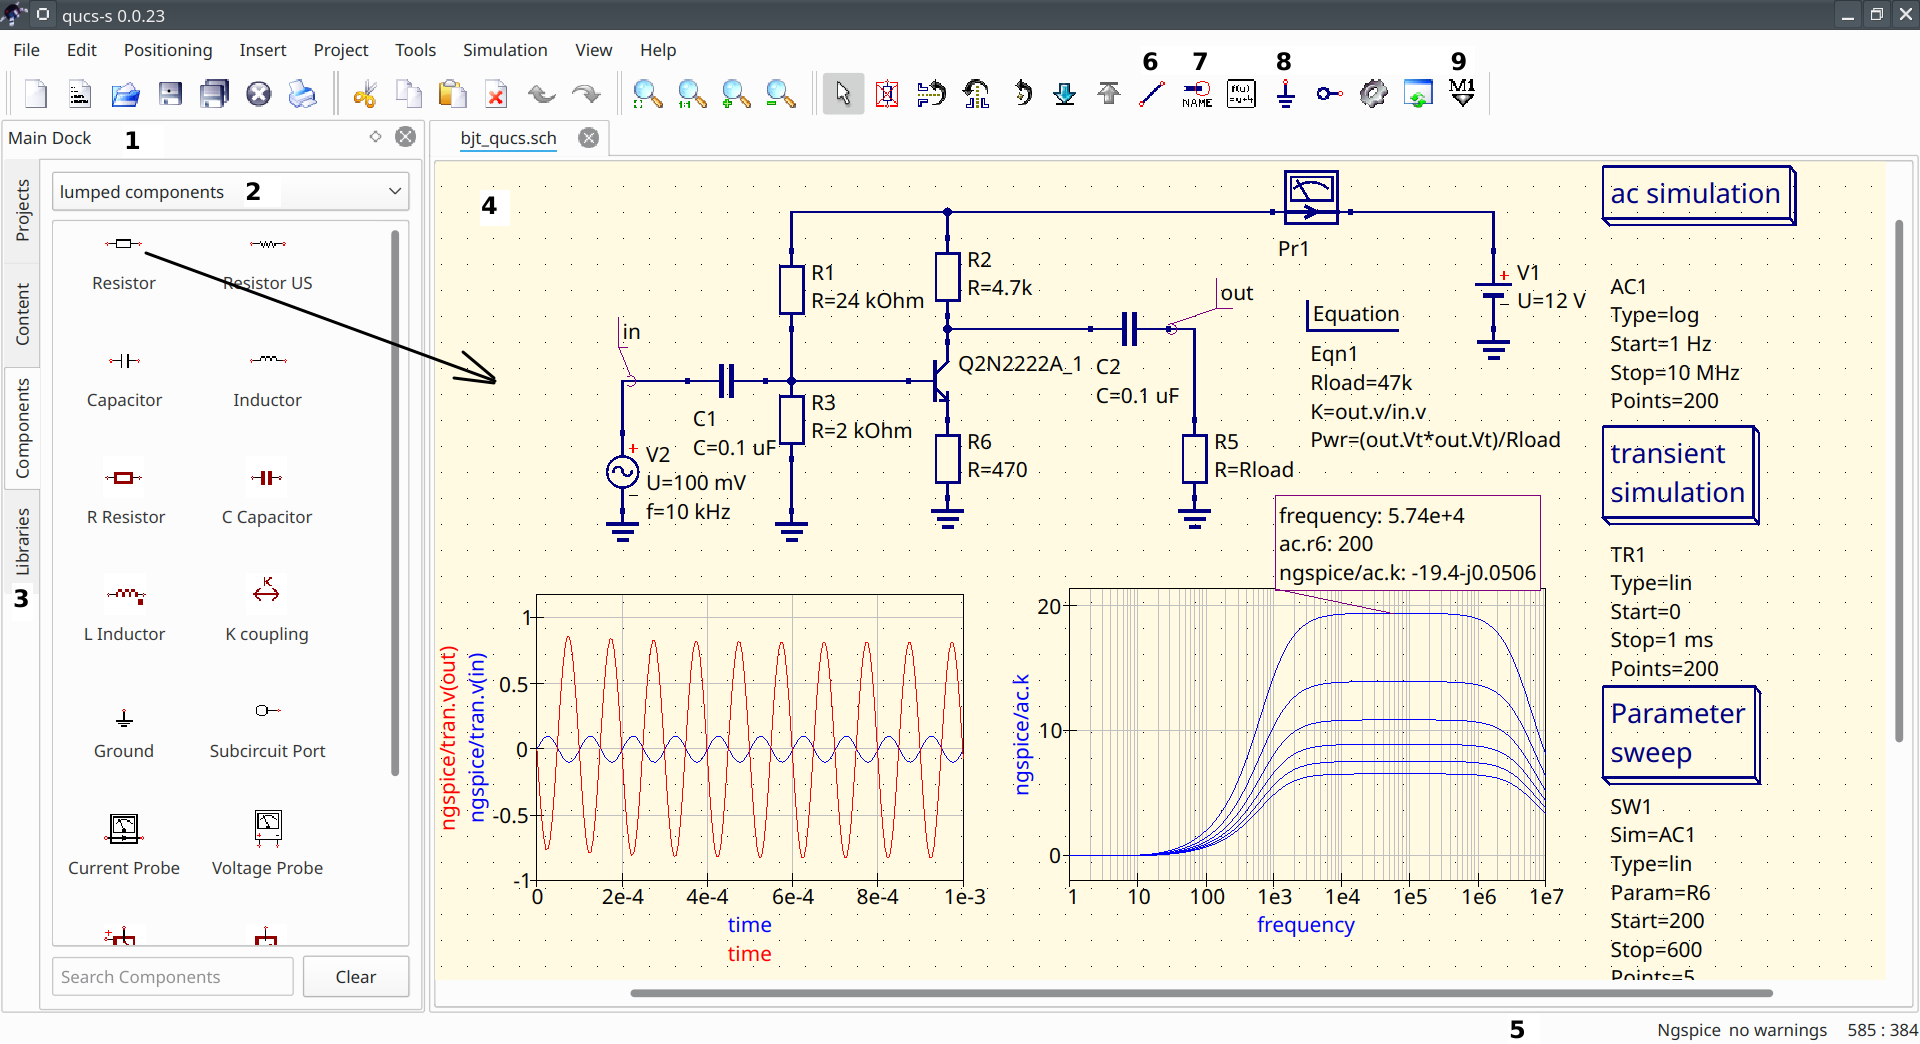
\includegraphics[width=\textwidth]{img/mainwin.png}
  \end{center}
  \caption{Qucs-S main window. See text for explanations} \label{fig:mainwin}
\end{figure}

The dock on the left side has four tabs (3): \emph{Projects}, \emph{Content}, \emph{Components}, and \emph{Libraries}. The \emph{Projects} tab is opened after the application start. It is empty, because there is no projects after the fresh installation. The \emph{Components} tab (see Fig. \ref{fig:mainwin}) contains a list of primitive devices available in Qucs. The components are divided into several categories (lumped devices, nonlinear devices, simulation, etc.). The categories could be selected from the drop-down list (2). The status bar is located on the bottom side of the main window. The active simulation kernel is displayed on the status bar (for example Ngspice on Fig.\ref{fig:mainwin}). 

The toolbar area is located on the top side of the main window below the main menu. Some important buttons are located on the toolbar. They are: \emph{Wire} (6), \emph{Node name} (7), \emph{Ground} (8), and \emph{Marker} (9).

Everything in Qucs-S is considered to be a component. The simulations, equations, and SPICE directives are also special components that could be found in dedicated categories in the component pallet. The diagrams are also special components and could be found in the \emph{diagrams} category in the drop-down list (2).

To place the component on schematic choose desired category from the drop-down list (2) (for example "lumped components") and click on the symbol (for example "Resistor"). Moving the mouse cursor into the working area (4) you are carrying a drawing of a resistor symbol. Pressing the right mouse button rotates the symbol, pressing the left mouse button places the component onto the schematic. 

The components properties could be edited using the properties dialog (Fig. \ref{fig:prop_dlg}) that is called from the context menu of the component or after the left mouse button double click. 

\begin{figure}[!ht]
  \begin{center}
    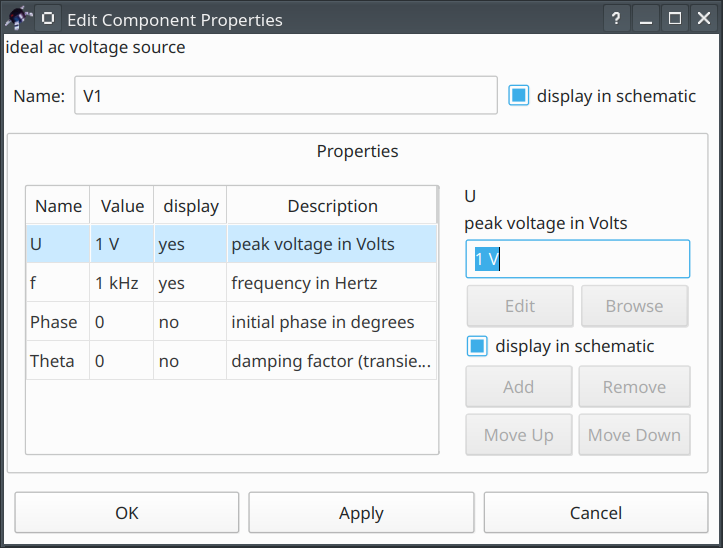
\includegraphics[width=0.45\textwidth]{img/prop_dlg.png}
  \end{center}
  \caption{Component properties dialog} \label{fig:prop_dlg}
\end{figure}

\section{Step by step guide how to setup an analog simulation}

\subsection{AC and transient simulation}

Let's simulated an RC-circuit using Qucs-S with Ngspice backend. The schematic is shown in the Fig. \ref{fig:rc}. Let's perform the AC and transient simulations and plot the magnitude response of the circuit and the waveforms on the input and output nodes. Perform the following steps to draw the schematic and setup the simulation. 

\begin{figure}[!ht]
  \begin{center}
    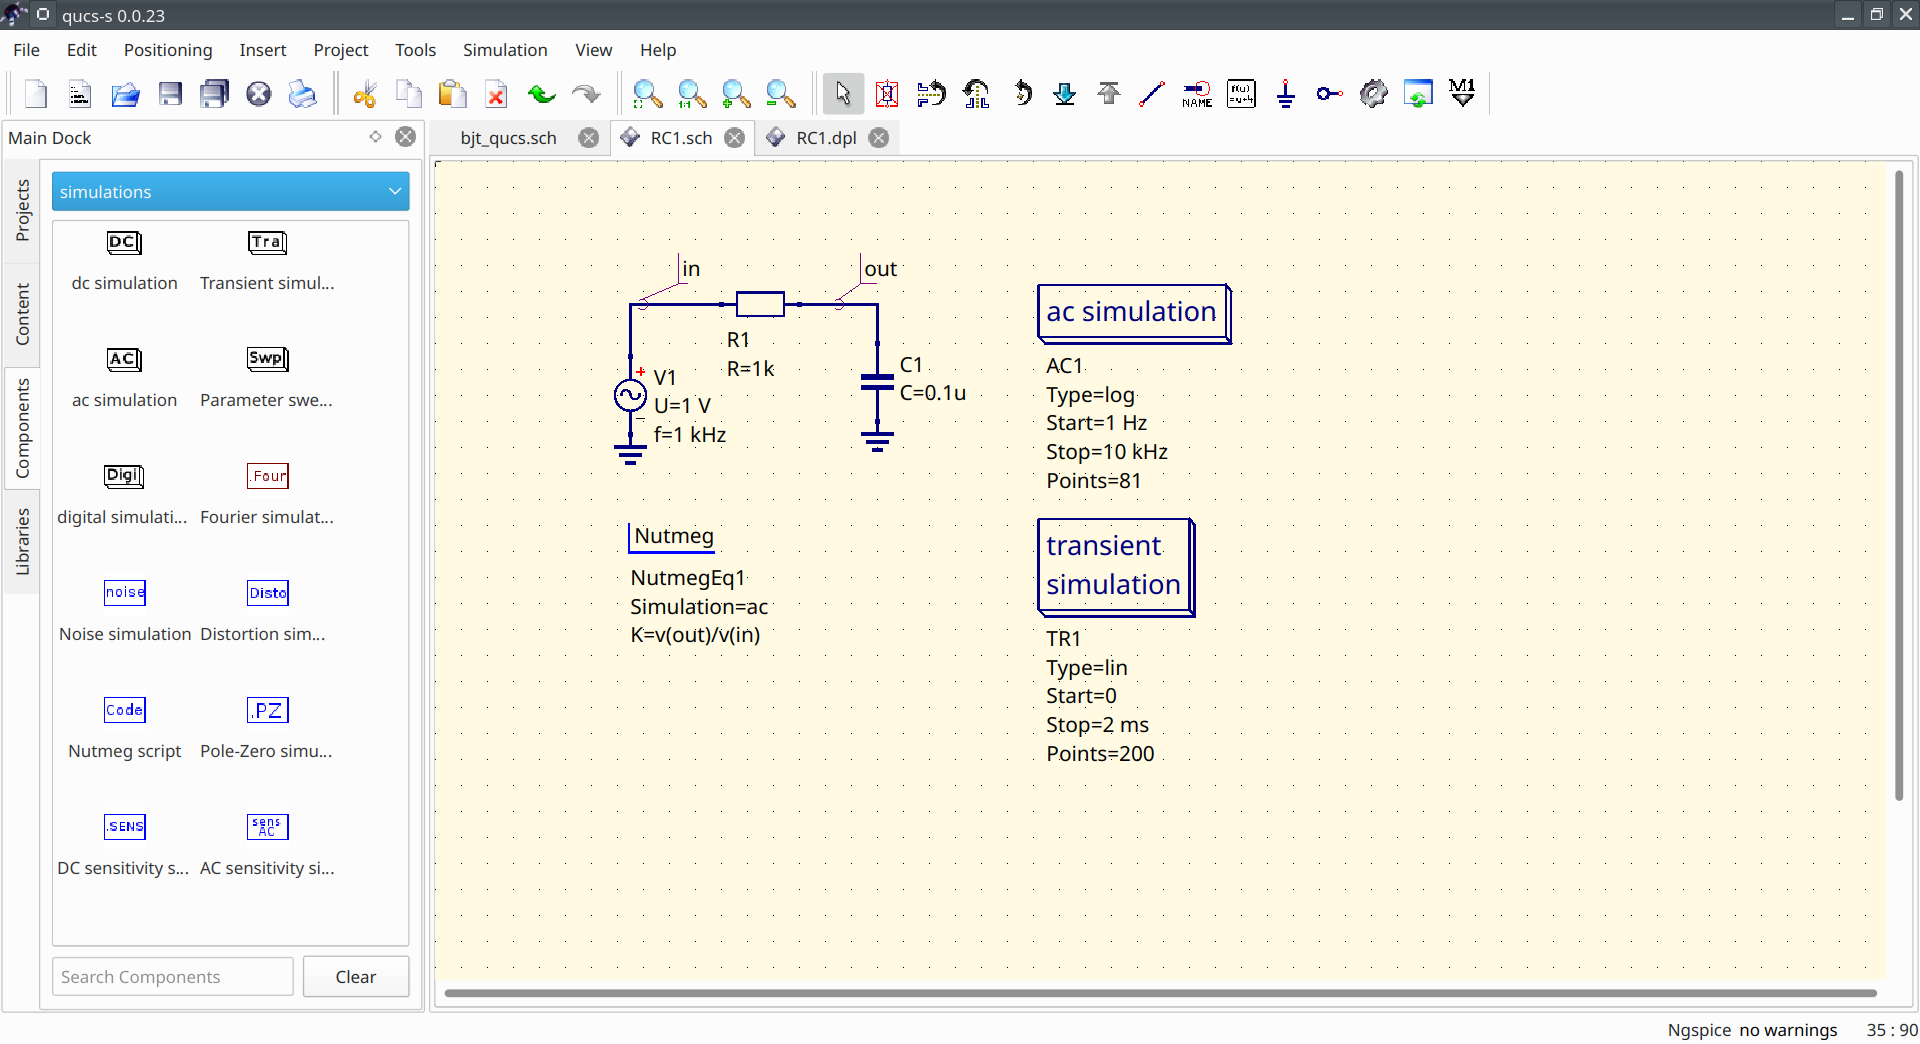
\includegraphics[width=\textwidth]{img/rc.png}
  \end{center}
  \caption{RC-circuit in Qucs-S} \label{fig:rc}
\end{figure}


\begin{itemize}
 \item \textbf{Step 1:} place components on the schematic and set their properties as show in the Fig. \ref{fig:rc}. We need resitor, capacitor (both could be found in the \emph{lumped devices} category) and AC voltage source (from \emph{sources} category). The ground and wires could be taken from the application tool bar (see Fig. \ref{fig:mainwin}) using the buttons (6) and (8). 
 
 \item \textbf{Step 2:} place simulations on the schematic. We need AC simulation and Transient simulation. Both could be taken from the \emph{simulations} category (see Fig. \ref{fig:rc}). The procedure is same as for usual components. Setup the properties of the simulations as shown in the Fig. \ref{fig:rc}. A special dialog window opens upon the double click on the simulation device (Fig. \ref{fig:dlg_sim}). For AC simulation enter the start (1 Hz) and stop (10 kHz) frequencies and select the logarithmic sweep type. For transient simulation enter the stop time (2 ms) and points number (200 points). 
 \begin{figure}[!ht]
  \begin{center}
    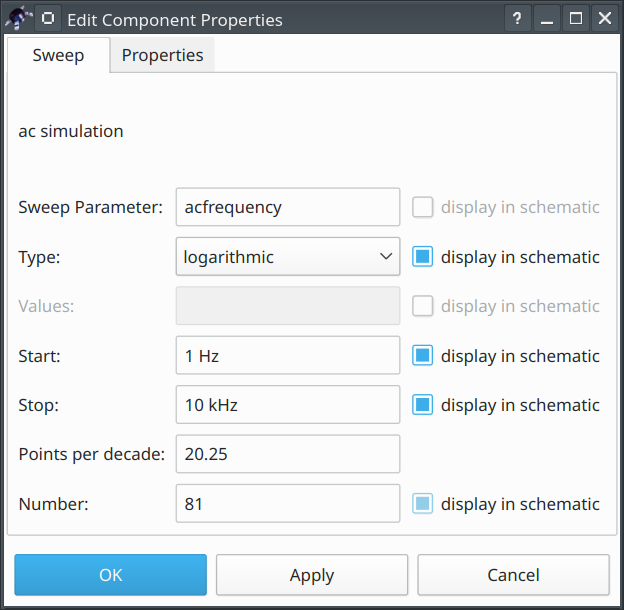
\includegraphics[width=0.45\textwidth]{img/dlg_sim.png}
  \end{center}
  \caption{Simulation properties dialog} \label{fig:dlg_sim}
\end{figure}
 
 \pagebreak[4]
 
 \item \textbf{Step 3:} place the node labels \verb|in| and \verb|out| using the button (6) on the toolbar (see Fig. \ref{fig:mainwin}). The node name could be set in a special dialog window (Fig. \ref{fig:nod_lbl}). 
 \begin{figure}[!ht]
  \begin{center}
    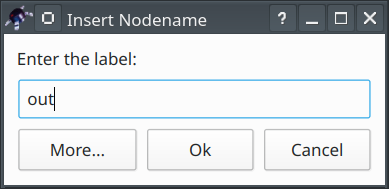
\includegraphics[width=0.4\textwidth]{img/nod_lbl.png}
  \end{center}
  \caption{Node label setup dialog} \label{fig:nod_lbl}
\end{figure}
 
 \item \textbf{Step 4:} Place equation for the magnitude response $K=V_{out}/V_{in}$ on the schematic. Equation is the special component called \emph{Nutmeg equation} that could be found in the \emph{spice specific sections} category. The full SPICE syntax for mathematical functions and node names is supported. Refer to Ngspice manual for more details. The simulation should be specified for each Nutmeg equation. We will calculate the magnitude response for the AC simulation only and therefore we need to enter \verb|ac| as the first property for this device as shown on the Fig. \ref{fig:eq}.
  \begin{figure}[!ht]
  \begin{center}
    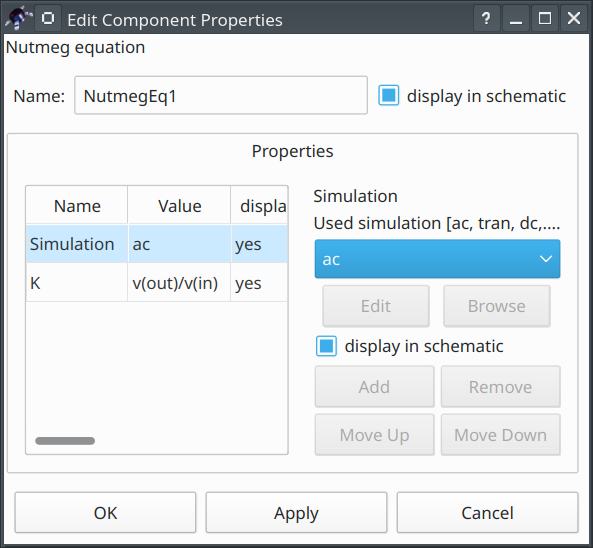
\includegraphics[width=0.4\textwidth]{img/nutmeg_eq.png}
  \end{center}
  \caption{Equation setup dialog} \label{fig:eq}
\end{figure}
 
 \item \textbf{Step 5:} Save the schematic document as the file with the \verb|*.sch| extension using the \textit{File} \verb|->| \textit{Save as} menu or press the \verb|Ctrl-S| shortcut. The schematic is ready for the simulation now.
 
 \item \textbf{Step 6:} simulate the schematic. Press the \textit{Simulation} \verb|->| \textit{Simulate} or press the F2 hotkey on the keyboard. The dialog window containing the simulator log messages will appear shortly (Fig. \ref{fig:sim_dlg}). This dialog window contains the simulation console where the messages from the Ngspice are shown. 
 
 It should report that the simulation finished without errors. If you see error messages check your schematic and application settings. After the Ngspice reports about the finished simulation, close this window clicking the \emph{Exit} button. Now the diagrams could be added on schematic field. It is also possible to save the netlist file from this dialog
 .
  \begin{figure}[!ht]
  \begin{center}
    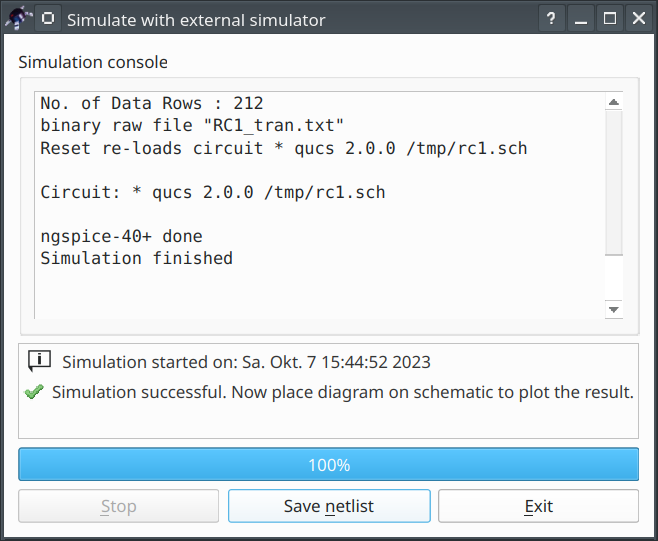
\includegraphics[width=0.4\textwidth]{img/sim_dlg.png}
  \end{center}
  \caption{Simulation dialog} \label{fig:sim_dlg}
  
\end{figure}

\item \textbf{Step 7:} place diagrams on the schematic (Fig. \ref{fig:rc_dpl}). We need two cartesian diagrams for magnitude response and transient waveforms. The diagrams are also special components that could be found in the \emph{diagrams} category. The traces could be selected in the special diagram properties dialog (Fig. \ref{fig:diagr_dlg}). Select the \verb|ac.k| traces for one diagram and \verb|tran.v(in)| and \verb|tran.v(out)| traces for another diagram. It is also possible to setup the axis limits and type and the color scheme for the diagram. Select logarithmic X-axis for the magnitude response graph using the settings in the \emph{Properties} tab. The markers could be placed on graphs using the button (9) from the toolbar (Fig. \ref{fig:mainwin}). The position of the marker could be adjiusted using the arrow keys on the keyboard. 

  \begin{figure}[!ht]
  \begin{center}
    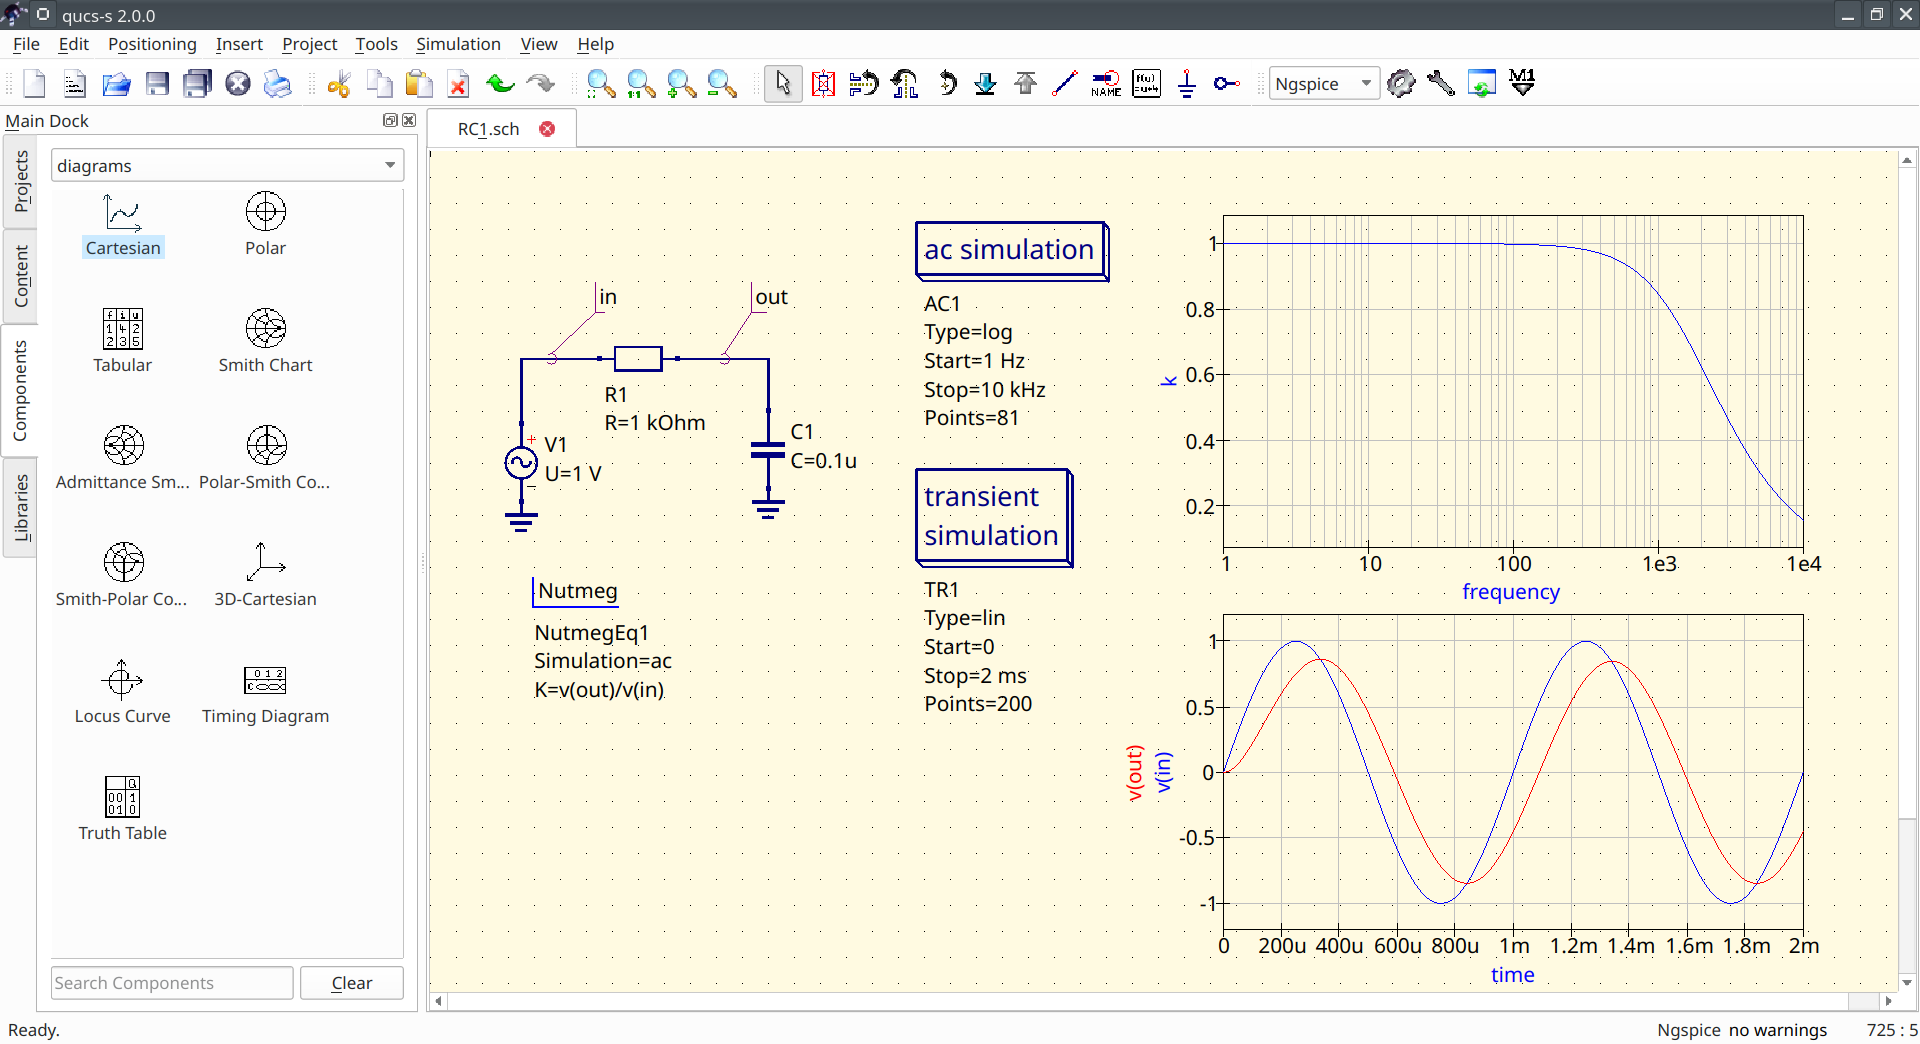
\includegraphics[width=\textwidth]{img/rc_dpl.png}
  \end{center}
  \caption{Schematic with two diagrams added} \label{fig:rc_dpl}
  \end{figure}
  
    \begin{figure}[!ht]
  \begin{center}
    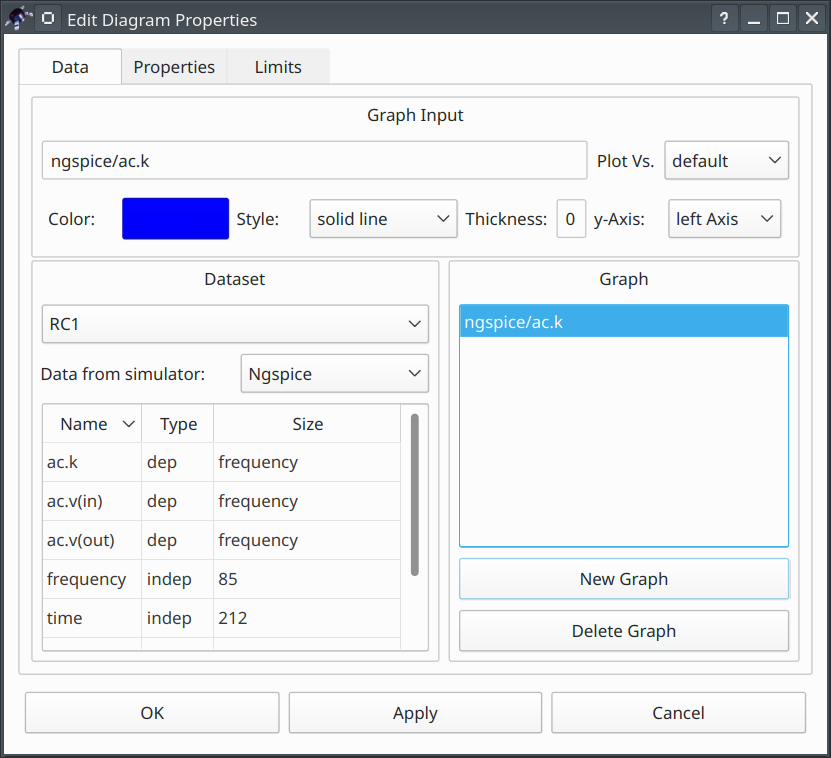
\includegraphics[width=0.4\textwidth]{img/diagr_dlg.png}
  \end{center}
  \caption{Diagram properties dialog} \label{fig:diagr_dlg}
  \end{figure}
  
\end{itemize}


\subsection{DC analysis} \label{sec:dc}

Qucs-S unlike Qucs has no special DC simulation mode. If only \emph{DC 
simulation} component is placed on the schematic no simulation will be launched 
and error message will be shown. This component is kept for backward 
compatibility with old Qucs schematics.

But there exists two modes of the DC simulation:

\begin{itemize}
 \item Show operating point directly on the circuit. This mode is activted when 
pressing F8 keyboard shortcut or using \emph{Simulation->Show bias} menu 
entry. See the Fig. \ref{fig:rdiv_f8} for example of such simulation.
 \item DC sweep mode. You need to insert \emph{Parameter sweep} simulation 
component and attach it to the DC simulation. This simulation mode could be 
used for plotting IV-curves or getting table output. See the Fig. 
\ref{fig:rdiv_dc} for example of this simulation. 
\end{itemize}


\begin{figure}[!ht]
    \begin{center}
        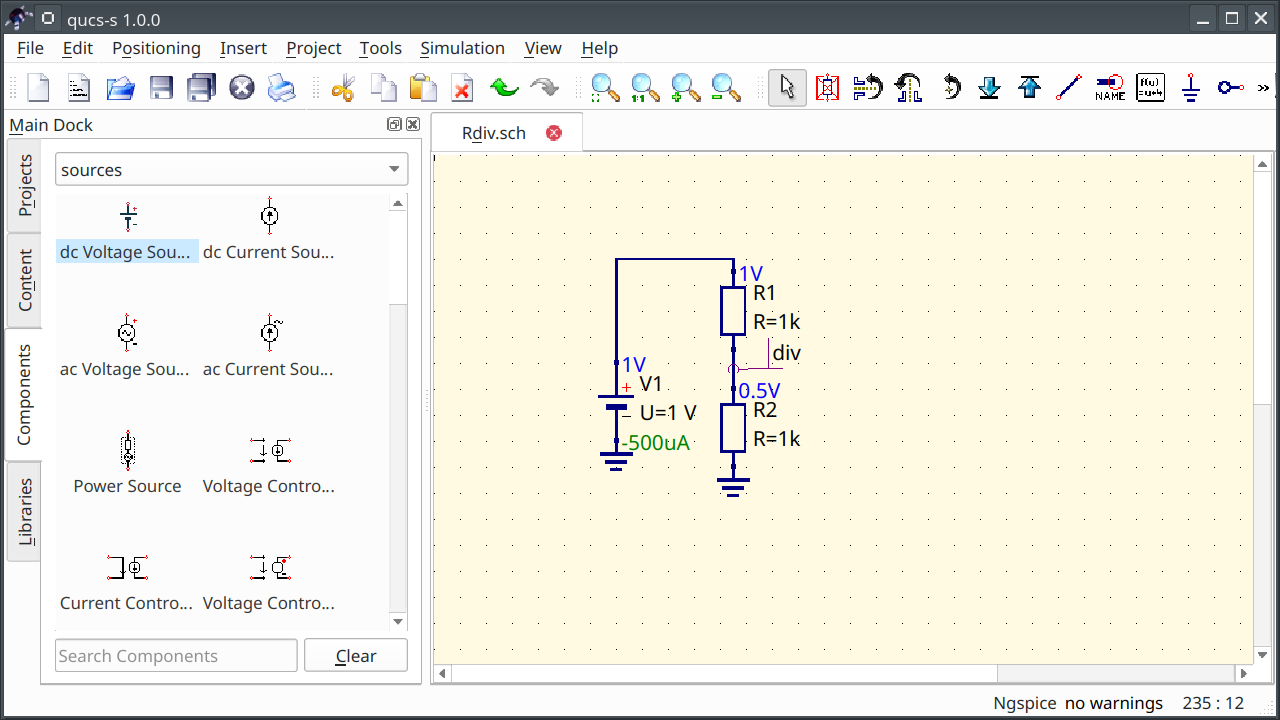
\includegraphics[width=0.8\textwidth]{img/rdiv_f8.png}
    \end{center}
    \caption{Operating point simulation of the voltage divider} 
\label{fig:rdiv_f8}
\end{figure}


\begin{figure}[!ht]
    \begin{center}
        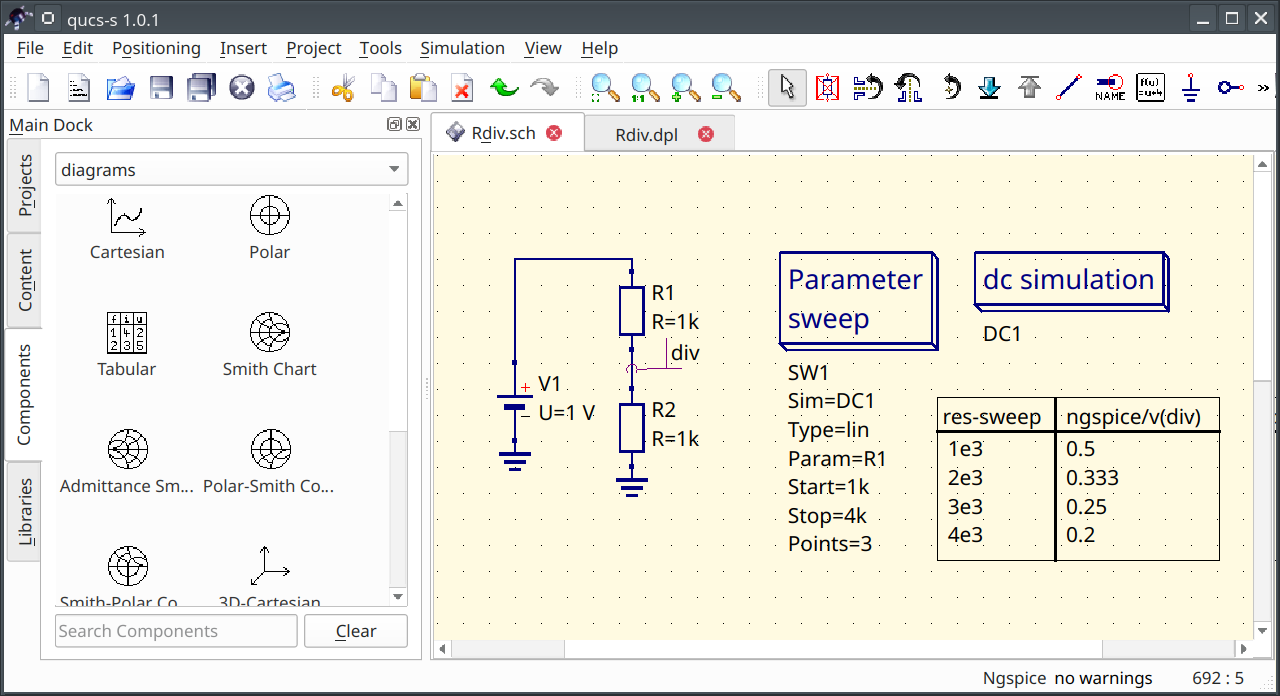
\includegraphics[width=0.8\textwidth]{img/rdiv_dc.png}
    \end{center}
    \caption{Using DC sweep to get table output of the resistive divider 
voltage} 
\label{fig:rdiv_dc}
\end{figure}

\section{Parameter sweep}

\subsection{Device sweep}

Parameter sweep is defined as the special simulation type that is attached to any other simulation. Let's consider an example
and attach parameter sweep to the circuit shown in the Figure \ref{fig:rc}. We will see the influence of the resistance of
the RC-circuit on the cutoff frequency. 

\textbf{Important note:} unlike Qucs before version 0.0.20, Qucs-S doesn't support the sweep of variables directly. Legacy Qucs schematics using variable sweep will not work. Parameter sweep supports only device sweep. Resistor, capacitor or source are accepted.  

Perform the following steps to add parameter sweep:

\begin{itemize}
 \item \textbf{Step 1:} Place parameter sweep component on the schematic sheet (Figure \ref{fig:rc_parsw}). 
 The \emph{Parameter sweep} device could be found in the \emph{simulations} group. 
 
    \begin{figure}[!ht]
        \begin{center}
            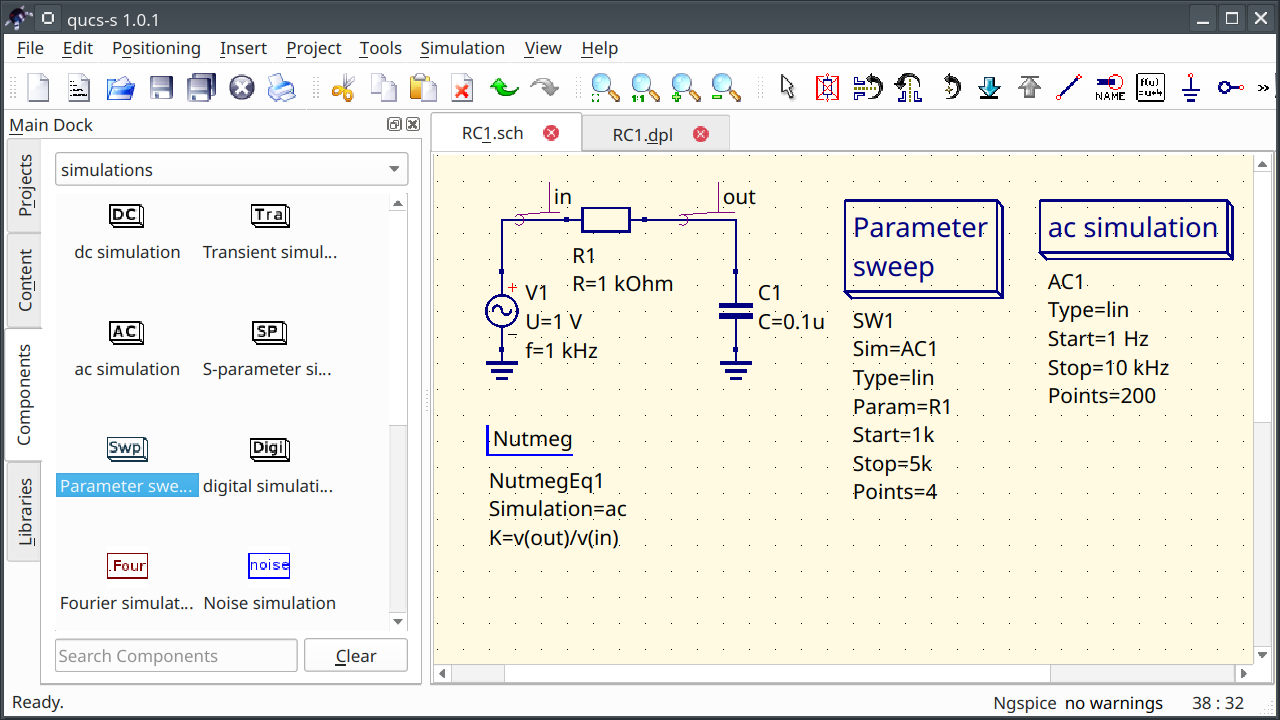
\includegraphics[width=0.8\textwidth]{img/rc_parsw.png}
        \end{center}
        \caption{Adding parameter sweep on the schematic} 
    \label{fig:rc_parsw}
    \end{figure}

\item \textbf{Step 2:} Set the properties of the parameter sweep simulation. After the double click the dialog window will be 
opened (Figure \ref{fig:parsw}). The \emph{Simulation} drop-down list is the the name of simulation component to which the parameter sweep is attached. For our example we need to select the \verb|AC1| simulation from the drop-down list, because we attaching the parameter sweep to the AC simulation. The \emph{Sweep parameter} input field is the \textbf{device} name. Variables or other objects 
name are not acceptable here! Enter the \verb|R1| device name here. The \emph{Start}, \emph{Stop}, \emph{Step}, and \emph{Number} input fields serve for the definition of the sweep range. We will sweep the \verb|R1| value from 1 kOhm to 5 kOhm and take 4 sweep points. 

    \begin{figure}[!ht]
        \begin{center}
            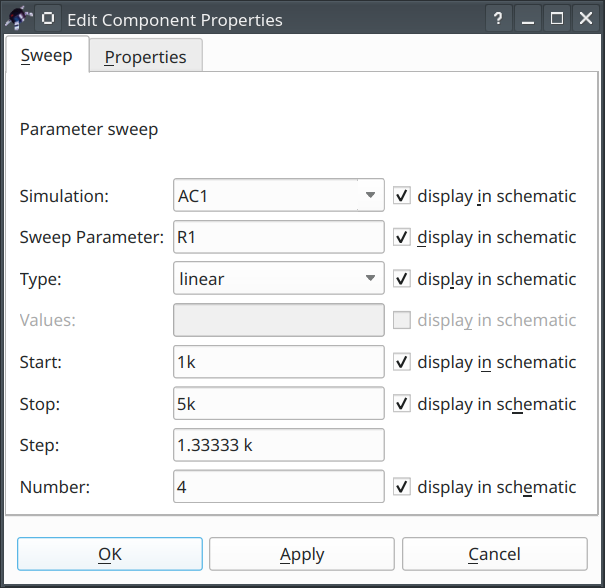
\includegraphics[width=0.5\textwidth]{img/parsw_dlg.png}
        \end{center}
        \caption{Setting parameter sweep properties} 
    \label{fig:parsw}
    \end{figure}
    
\item \textbf{Step 3:} Run the simulation and place the diagrams as for usual simulation (Figure \ref{fig:parsw_mr}). You should see the family of the curves. You may place a marker on the diagram and move it between the sweep curves with \emph{Arrow Up} and \emph{Arrow Down} keys.  
    
        \begin{figure}[!ht]
        \begin{center}
            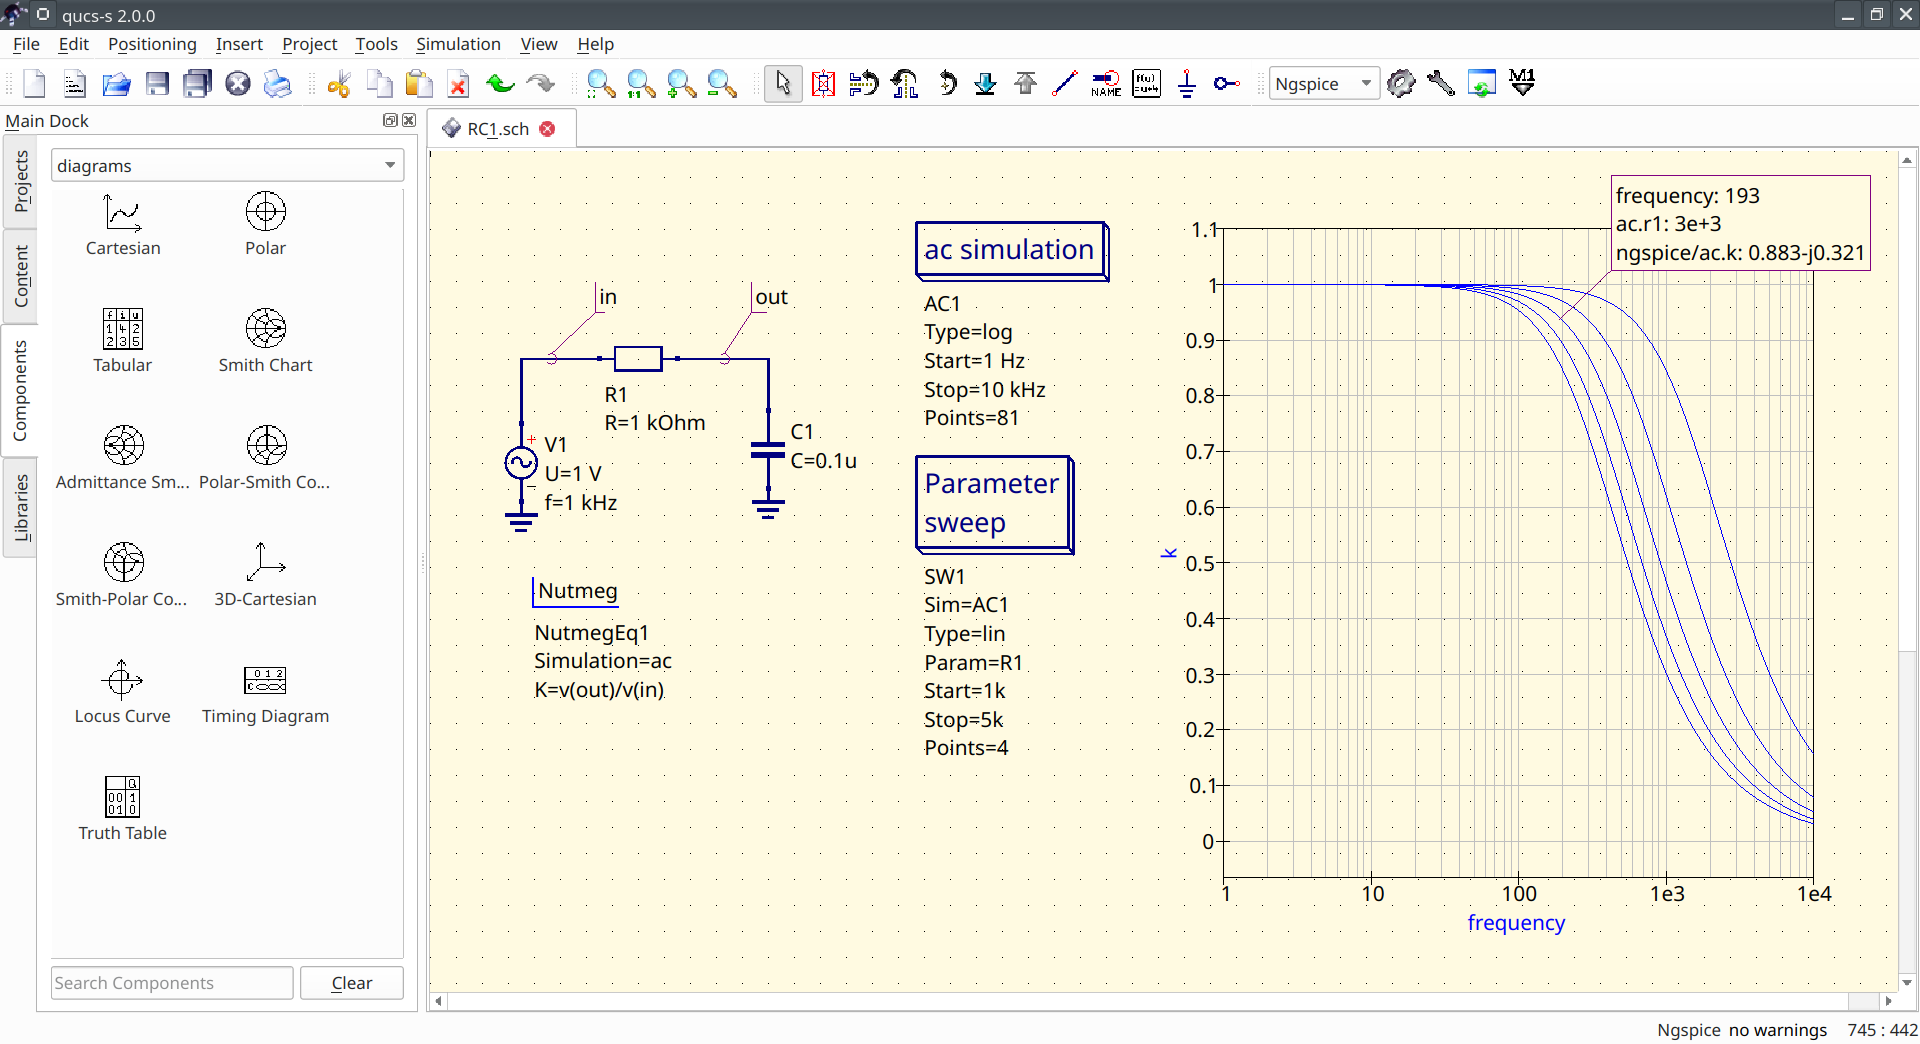
\includegraphics[width=0.8\textwidth]{img/parsw_mr.png}
        \end{center}
        \caption{Magnitude response of the RC-circuit with the parameter sweep} 
    \label{fig:parsw_mr}
    \end{figure}
    
\end{itemize}


\subsection{DC sweep}

DC sweep simulation takes place when parameter sweep is attached to the DC simulation. Such simulation mode is explained in
the Section \ref{sec:dc}. DC sweep only accepts device name (resistor or source) as the sweep parameter name. This simulation mode
usually serves for obtaining the IV-curves. 

\subsection{Variable sweep}

The recent version of the Ngspice support sweeping of the varibles. The variable should be defined using the \verb|.PARAM| 
statement (available at the \emph{SPICE specific sections} group). Qucs-S doesn't create the variable automatically. Refer to the schematic shown in the Figure \ref{fig:rc_parsw_var} for the example of such simulation mode.

        \begin{figure}[!ht]
        \begin{center}
            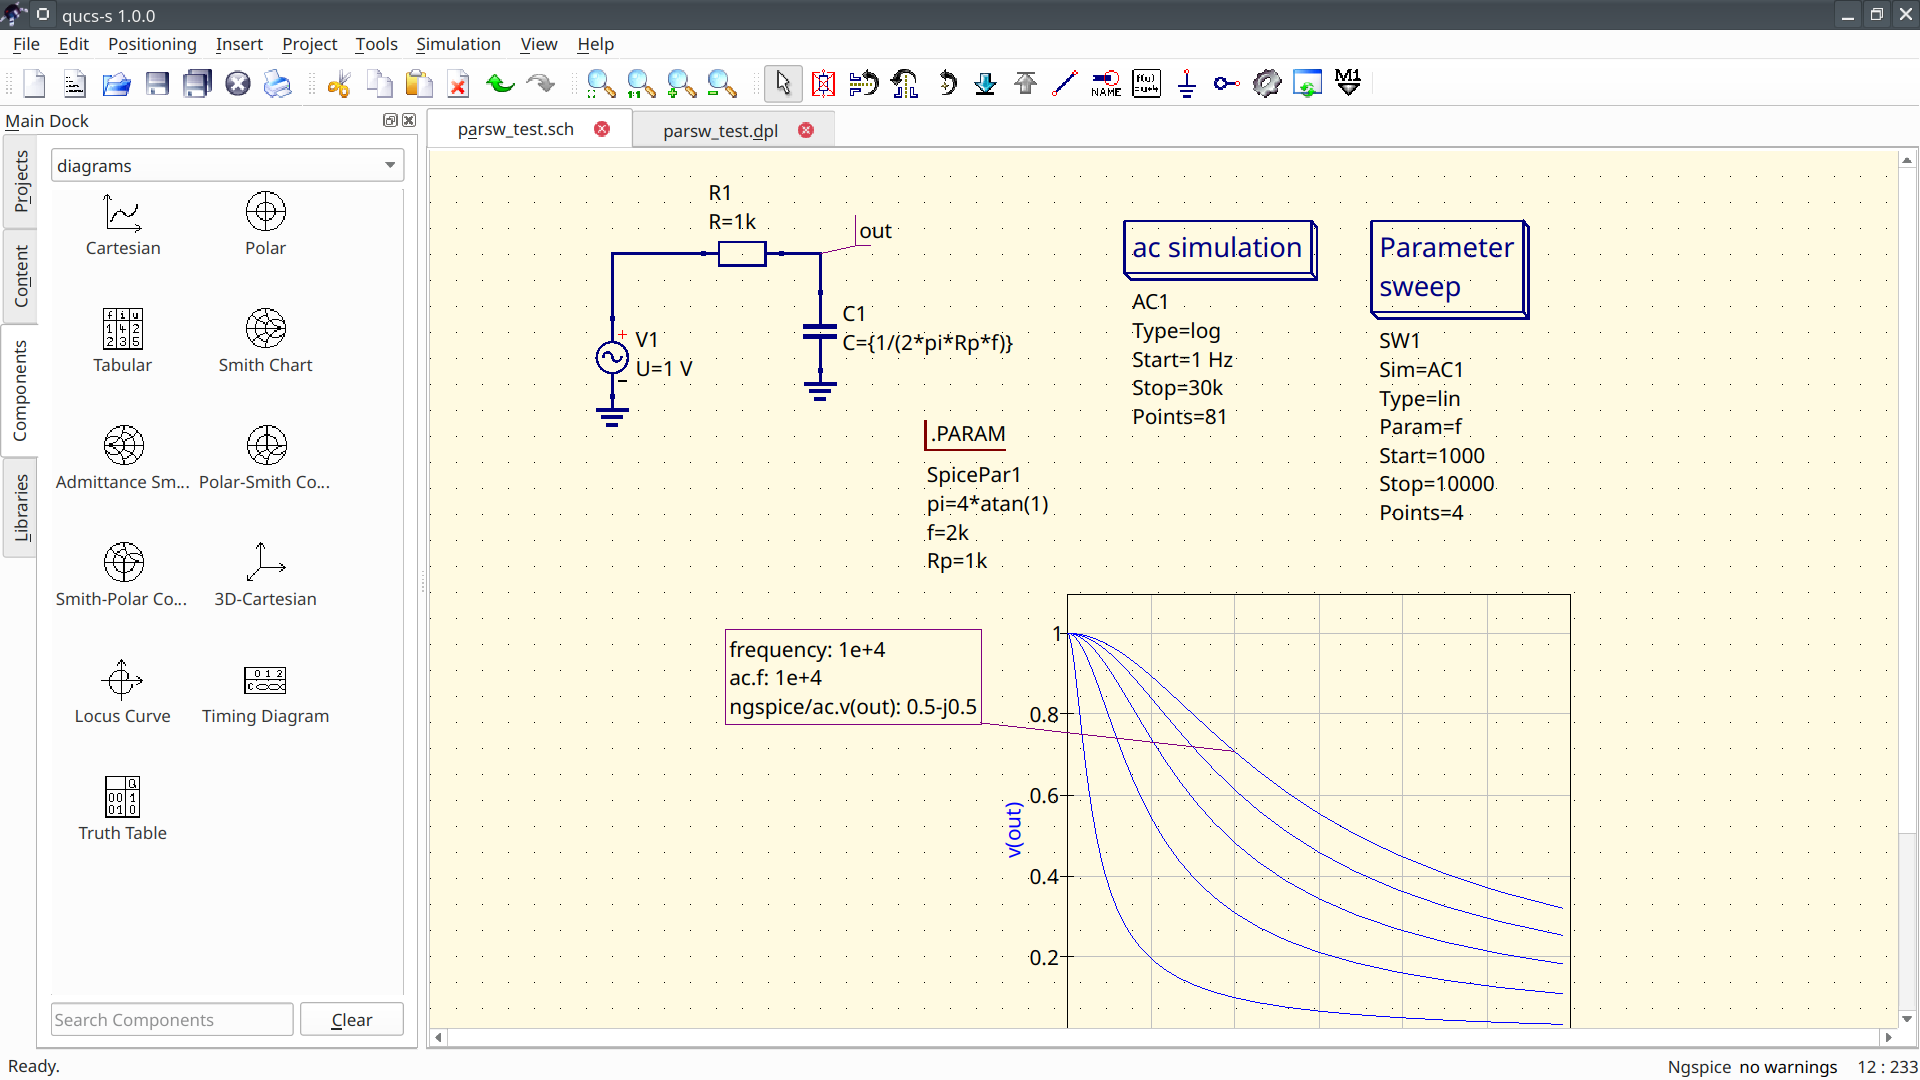
\includegraphics[width=0.8\textwidth]{img/rc_parsw_var.png}
        \end{center}
        \caption{Magnitude response of the RC-circuit with the parameter sweep} 
    \label{fig:rc_parsw_var}
    \end{figure}
    
\section{Digital simulation}

\subsection{Digital devices with analog model}

Digital devices including logic gates, flip-flops, and more complex devices could be found in the group \emph{Digital components}. Some of these devices have both analog and digital model. Ngspice simulation operates using XSPICE models. Here is the list of these devices:

\begin{itemize}
 \item Logic gates, inverter and buffer
 \item D-, JK-, T-flip-flops
 \item Digital source
\end{itemize}

The usage of these devices in analog simulation mode has no special requirements. The example shown in the Figure \ref{fig:logic_gen} illustrates the transient simulation of the RC oscillator circuit containing two inverter logic gates. The power supply voltage for digital devices should be set using the \verb|VCC| parameter with \verb|.PARAM| section.

    \begin{figure}
    \begin{center}
        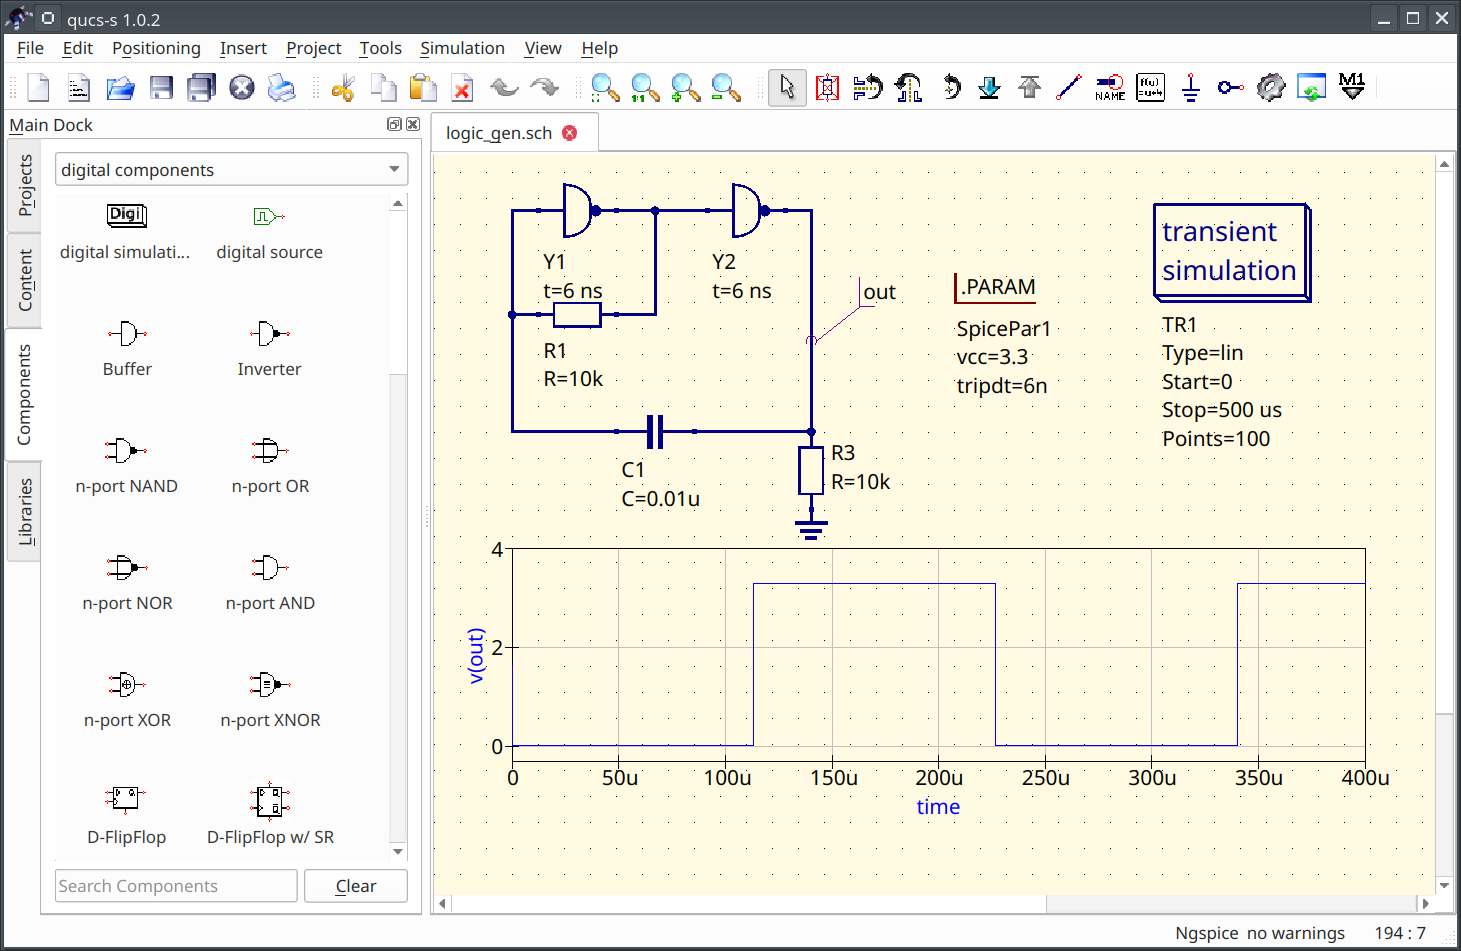
\includegraphics[width=0.8\textwidth]{img/logic_gen.png}
    \end{center}
    \caption{Oscillator example using logic gates} \label{fig:logic_gen}
    \end{figure}


\subsection{Digital simulation with Verilog/VHDL} \label{sec:digi}

The most of digital components except of the listed in the previous section doesn't contain analog SPICE model. These devices are  supported by digital simulation mode only. \textbf{Mixing digital and analog devices (like RCL) in one circuit is not supported!} You need to install one the following free backends to perform digital simulation

\begin{itemize}
 \item Icarus Verilog \verb|iverilog| \url{https://steveicarus.github.io/iverilog/}
 \item FreeHDL \url{http://freehdl.seul.org/}
\end{itemize}


Place on the schematic field a special device named \emph{Digital simulation} to switch Qucs-S to digital mode. Verilog or VHDL backend will be started automatically instead of SPICE if digital simulation is found in the schematic. User doesn't need to switch 
Qucs-S to the digital mode in the application settings. 

There are two modes of the digital simulation: truth table and timing diagram. An example of the digital simulation of the 2-bit decoder/demultiplexer is shown in the Figure \ref{fig:demux}. This simulation uses Verilog and timing diagram mode. 

    \begin{figure}
    \begin{center}
        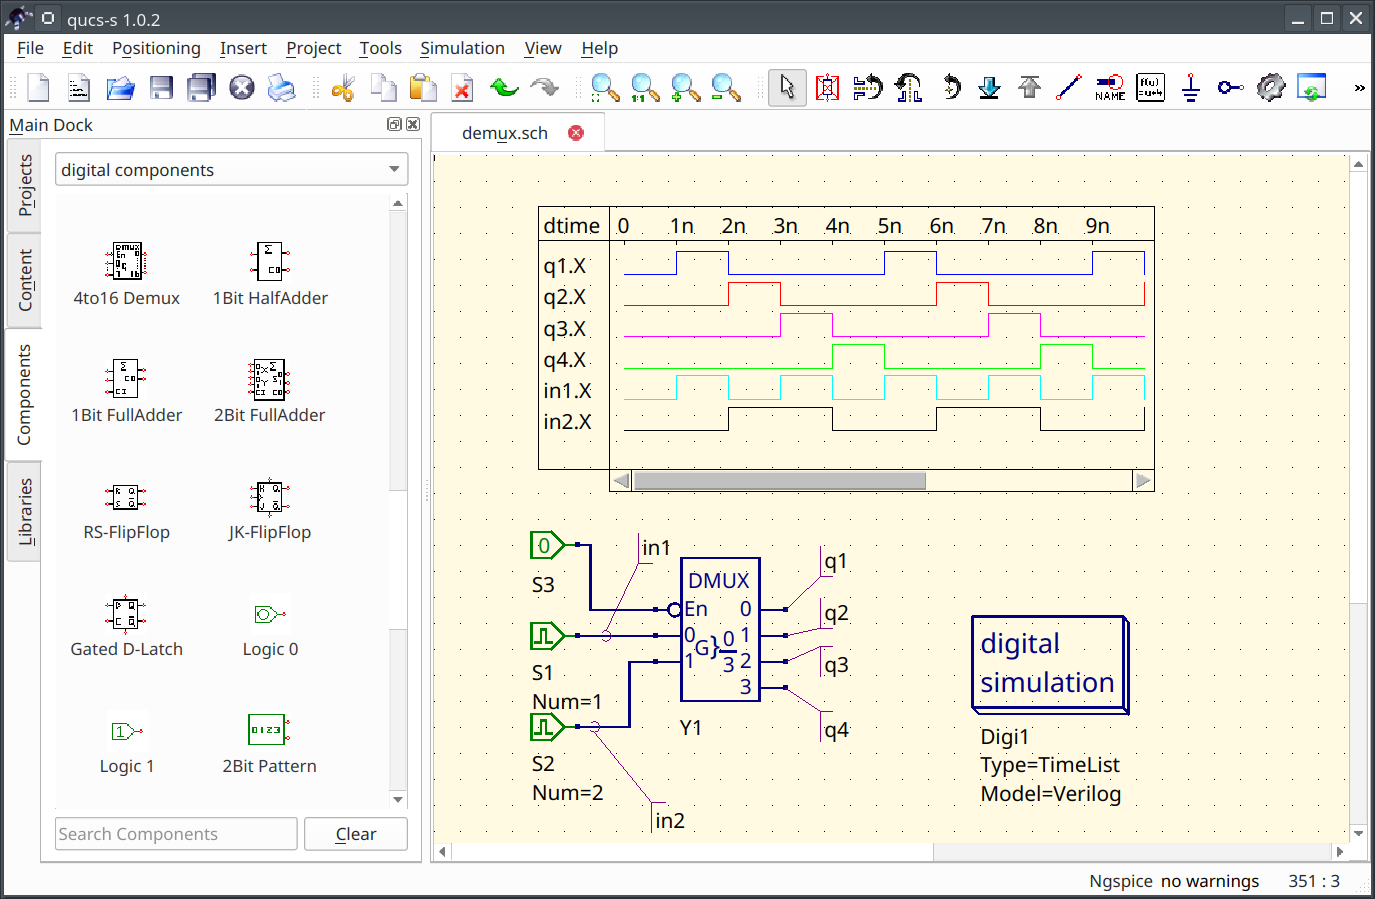
\includegraphics[width=0.8\textwidth]{img/demux.png}
    \end{center}
    \caption{Simulation of the digital circuit with iverilog} \label{fig:demux}
    \end{figure}

\section{Quick switching of the simulation kernel} \label{sec:quick_sw}

\subsection{Quick simulator selection}

Qucs-S supports a quick switching of the simulation kernel since the version 2.0.0. Application restart is not required anymore to apply this setting. The simulator could be selected at any time using the drop-down list on the toolbar Figure \ref{fig:sim_switch}. The simulator location must be configure using the application settings dialog Figure \ref{fig:sim_setup} and the specified simulator executable binary must exist. Otherwise the simulator will be not shown in the drop-down list on the toolbar and not available for selection. The list of the supported simulation kernels could be found in the section \ref{sec:intro}.

Also keep in mind that Qucs-S distribution doesn't provide any simulation kernels and simulators must be installed separately. If you are using Linux DEB package, the Ngspice will be installed automatically as the package dependency. This selection affects only analog simulation. The digital simulation kernel will be executed automatically if the schematic contains the digital simulation (see the section \ref{sec:digi}).  

    \begin{figure}
    \begin{center}
        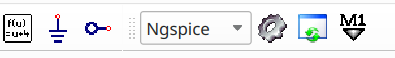
\includegraphics[width=0.8\textwidth]{img/sim_switch.png}
    \end{center}
    \caption{Simulator choose drop-down list} \label{fig:sim_switch}
    \end{figure}

\subsection{Incompatible components}
    
Some of devices may be incompatible with the selected simulation kernel. For example, microstrip lines are designed for Qucsator and are not available with Ngspice. Such devices will be not available for insertion in the schematic and will be grayed out (see Figure \ref{fig:grey}) on the schematic view. An appropriate warning will be shown if the user tries to simulate the schematic containing incompatible devices.

    \begin{figure}
    \begin{center}
        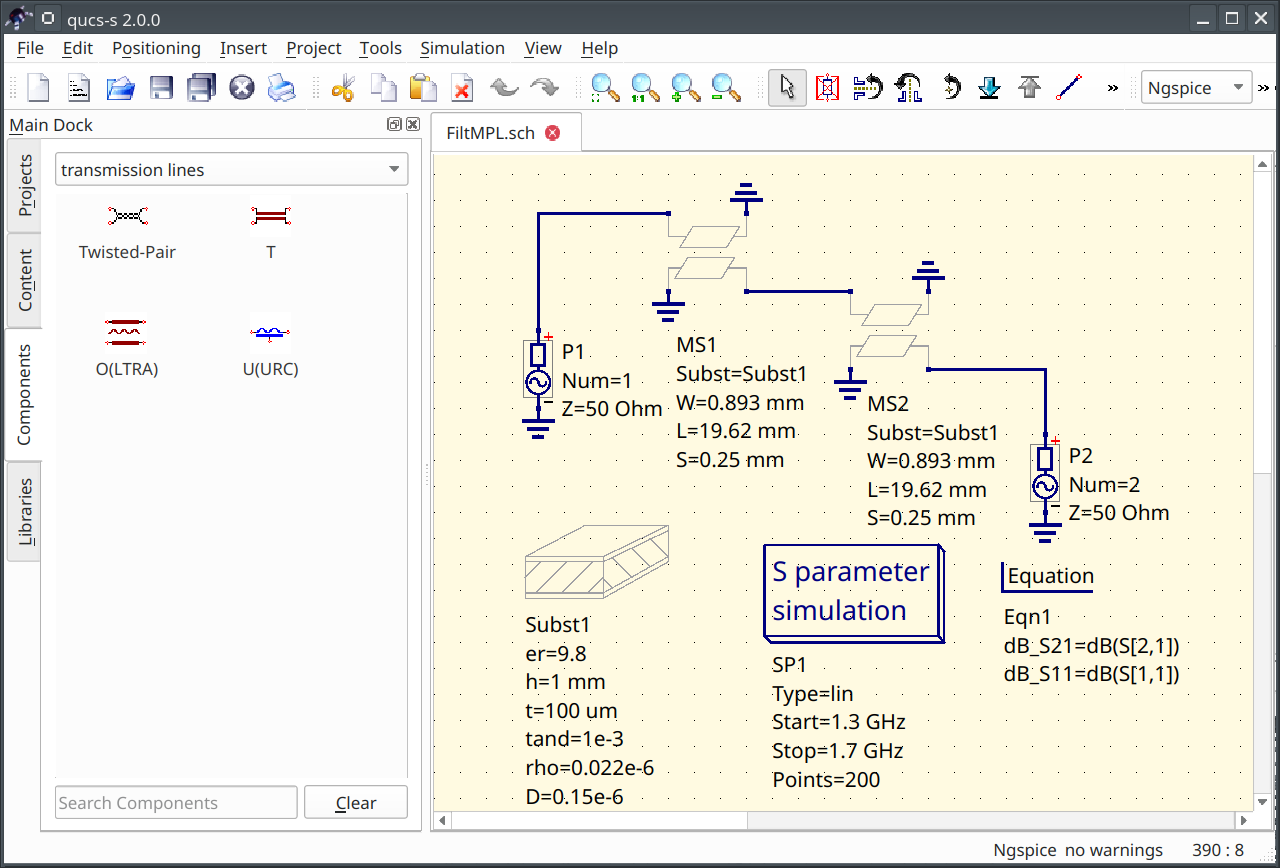
\includegraphics[width=0.8\textwidth]{img/ms_grey.png}
    \end{center}
    \caption{Schematic containing incompatible devices} \label{fig:grey}
    \end{figure}

\section{List of mathematical functions supported by Nutmeg equation}

The full list of the mathematical functions supported by Nutmeg equations could be found at the section 17.2 of the Ngspice manual. The next table shows the most frequently used functions. The input of all functions listed in the next table is a single vector representing voltage or current. Refer to the section 17 of the Ngspice manual for detailed description and information on additional functions.

\begin{table}[!ht]
\caption{The list of the most frequently used Nutmeg functions}
 \begin{tabularx}{\textwidth}{|r|X|}
\hline
Function & Description \\
\hline
mag & Magnitude of vector (same as abs(vector)) \\
ph & Phase of vector. \\
cph & Phase of vector. Continuous values, no discontinuity at $\pm\pi$ \\
unwrap & Phase of vector. Continuous values, no discontinuity at $\pm\pi$ Real phase vector in degrees as input \\
real & The real component of vector \\
imag & The imaginary part of vector\\
conj & The complex conjugate of a vector \\
db & Decibels $20 \log_{10}()$ of the vector \\
abs & The absolute value of vector (same as mag) \\
integ & Integrates over the given vector (versus the real component of the scale vector) \\ 
deriv & Calculates the derivative of the given vector \\
vecd & Compute the differential of a vector \\
group\_delay & Calculates the group delay $-d\phi/d\omega$ \\
\hline
\end{tabularx}
\end{table}




\section{Conclusion}

In this tutorial it was considered how to perform a first start setup of the Qucs-S with the Ngspice backend and make an AC and Transient simulation of the simple RC circuit. It was shown how to add postprocessor equations and waveforms plot. Refer to official Qucs-S and Ngspice documentation to learn more advanced simulation techniques. 



\end{document}


